% !TeX root = ../libro.tex
% !TeX encoding = utf8

\setchapterpreamble[c][0.75\linewidth]{%
	\sffamily
	En este capítulo abordaremos los detalles más importantes de la implementación realizada en C++ de los algoritmos. Así como el cálculo de tiempos de ejecución para comparar con la complejidad teórica calculada en el \autoref{ch:cuarto-capitulo}. Para mostrar los tiempos de ejecución y los ajustes a las funciones de complejidad se utilizará Gnuplot \cite{alma991008609239704990}.
	\par\bigskip
}
\chapter{Experimentación}\label{ch:quinto-capitulo}

Toda la implementación está disponible en el siguiente repositorio de \href{https://github.com/PabloC01/TFG}{GitHub}\footnote{Dirección url: https://github.com/PabloC$01$/TFG}. La implementación se encuentra en la carpeta \textit{Codigo}, dividida a su vez en $4$ carpetas:

\begin{itemize}
	\item \textit{FUENTES}: contiene los archivos fuente con el propio código y el archivo \textit{MAKEFILE}.
	\item \textit{Grafos}: contiene archivos con la representación de los grafos que se muestran a lo largo de la sección 3.
	\item \textit{Resultados}: contiene los archivos de texto con los tiempos de ejecución obtenidos.
	\item \textit{bin}: contiene los programas ejecutable, así como el script de cálculo de tiempos y un archivo de texto \textit{LEEME} con instrucciones.
\end{itemize}

Para representar las estructuras necesarias para implementar los algoritmos se han utilizado los TDA más comunes de la STL de C++ \cite{alma991014010751904990}, como pueden ser la clase \textit{vector<>} o \textit{queue<>}, en función de las necesidades requeridas por las diferentes estructuras a implementar.

\section{Clase Grafo}

Utilizaremos esta clase para poder representar grafos en C++. Está implementada en los archivos \textit{Grafos.h} y \textit{Grafos.cpp}, en ellos se implementa la propia clase, que consiste de una matriz que se utilizará como matriz de adyacencia, otra matriz que se utilizará como lista de adyacencia y otras variables asociadas al grafo como el número de nodos. Además se implementa una función para construir la lista de adyacencia a partir de la matriz de adyacencia, para poder construir los grafos de manera más simple. \\

También se implementan dos funciones para generar grafos de forma aleatoria, para ello simplemente generamos aristas aleatorias hasta llenar el número de aristas del grafo, que se calculan de la siguiente manera a partir de la densidad del grafo:

$$|E| = |V|(|V| - 1)d$$

donde $d$ es la densidad del grafo, representada como número decimal, entre $0$ y $1$. \\

Como parte de la clase \textit{Grafo} se incluyen también constructores para poder guardar un grafo a partir de la matriz de adyacencia y atributos del grafo. También se ha implementado un constructor para guardar un grafo a partir de un archivo de texto, donde aparezcan primero los atributos del grafo y, depués, la matriz de adyacencica. Por último se incluye una función para mostrar la matriz de adyacencia del grafo y el número de nodos.

\section{Búsqueda en anchura}

Los dos algoritmos de Búsqueda en anchura están implementado en los archivos \textit{BFS.h} y \textit{BFS.cpp}. Por comodidad, se han utilizado dos vectores de la STL para guardar la distancia actual de un nodo y si ha sido explorado o no. No se han incluido estos atributos a la clase \textit{Grafo} para hacerla lo más simple posible, pues no todos los algoritmos utilizan estos atributos. \\

A parte de esto, como ya se comentó anteriormente, se ha utilizado el TDA \textit{queue<>} para simular la Cola en el algoritmo de búsqueda en anchura. Por último se ha utilizado la constante \textit{INT\_MAX} para simular el infinito.

\section{Dijkstra}

El algoritmo de Dijkstra está implementado en los archivos \textit{DJK.h} y \textit{DJK.cpp}. La implementación es igual a la búsqueda en anchura, salvo por el uso de la cola con prioridad. Para implementar dicha cola se ha utilizado el TDA \textit{priority\_queue<>}, creando para ello una clase \textit{comparador}, que compare dos nodos en función de su distancia actual almacenada en el vector de distancias.

\section{Bellman-Ford}

El algoritmo de Bellman-Ford está implementado en los archivos \textit{BF.h} y \textit{BF.cpp}. Por simplificar el código se ha incluido el código del proceso de relajación de una arista directamente al cuerpo del algoritmo, pues es el único algoritmo que utiliza dicho proceso. \\

A la hora de crear el vector de distancias, en este caso, en vez de utilizar la constante \textit{INT\_MAX}, se le ha restado una catidad arbitrariamente grande, pero bastante más pequeña que dicha constante. Esto es por un simple motivo, el condicional en la operación de relajación suma la distancia actual con el peso de la arista que se está relajando. En el caso de que la distancia actual sea \textit{INT\_MAX}, si le sumamos el peso, produce overflow, convirtiéndose en un número negativo, y, por tanto, rompiendo el algoritmo. Esto nunca sucede sin embargo en los dos algoritmos anteriores porque dicha comprobación sólo se realiza sobre nodos que han salido de la Cola, y a dichos nodos siempre se le modifica la distancia actual por una menor que \textit{INT\_MAX}.

\section{Multiplicación de matrices y Floyd-Warshall}

Estos algoritmos están implementados en los archivos \textit{Warshall.h} y \textit{Warshall.cpp}. La implementación de estos algoritmos ha sido algo más problemática y complicada que el resto. Principalmente debido a que la aritmética con el infinito hay que simularla mediante el uso de constantes y condicionales para separar casos en los que las variables son ``infinitas'' o no. \\

Además hay que construir la matriz inicial, pues partimos de la matriz de adyacencia, que no tiene los valores infinitos, necesarios para el funcionamiento de los algoritmos. \\

Los algoritmos de Floyd-Warshall y la Clausura Transitiva por otro lado han sido más sencillos de implementar, sin ningún contratiempo importante.

\section{Programas principales}

Se han creado dos programas principales, \textit{TFG.cpp} y \textit{Tiempos.cpp}. El primero ejecuta todos los algoritmos y muestra los resultados sobre un grafo aleatorio o un grafo almacenado en un archivo de texto. El segundo muestra el tiempo de ejecución del algoritmo pasado como parámetro, repitiendo la ejecución $10$ veces y calculando la media. \\

A continuación se muestra la salida del programa principal para cada algoritmo sobre el ejemplo con el que se explicó cada algoritmo.

\subsection{Resultado BFS}

\begin{figure}[!htb]
	\centering
	\begin{subfigure}{\linewidth}
		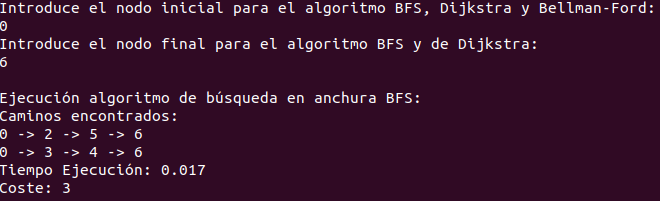
\includegraphics[width=14cm]{./Tiempos_Ejecucion/Ejecucion_BFS}
	\end{subfigure}
	
	\caption{Resultado de ejecución del algoritmo BFS con el grafo de la \autoref{fig:bfs-camino}.}
	\label{fig:resultado_BFS}
\end{figure}

\subsection{Resultado BFS Conexas}

\begin{figure}[!htb]
	\centering
	\begin{subfigure}{\linewidth}
		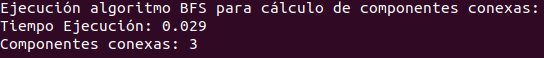
\includegraphics[width=12cm]{./Tiempos_Ejecucion/Ejecucion_BFS_C}
	\end{subfigure}
	
	\caption{Resultado de ejecución del algoritmo BFS Conexas con el grafo de la \autoref{fig:bfs-conexas}.}
	\label{fig:resultado_BFS_C}
\end{figure}

\subsection{Resultado Dijkstra}

Para este ejemplo los nodos $a$-$h$ son los nodos $0$-$7$ por lo que el camino obtenido se traduce como $a - c - e - f - h$.

\begin{figure}[!htb]
	\centering
	\begin{subfigure}{\linewidth}
		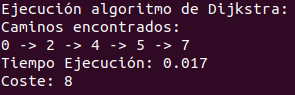
\includegraphics[width=6cm]{./Tiempos_Ejecucion/Ejecucion_DJK}
	\end{subfigure}
	
	\caption{Resultado de ejecución del algoritmo DJK con el grafo de la \autoref{fig:djk}.}
	\label{fig:resultado_DJK}
\end{figure}

\subsection{Resultado Bellman-Ford}

En este caso la numeración es la siguiente: $s:0$, $t:1$, $y:2$, $x:3$, $z:4$.

\begin{figure}[!htb]
	\centering
	\begin{subfigure}{\linewidth}
		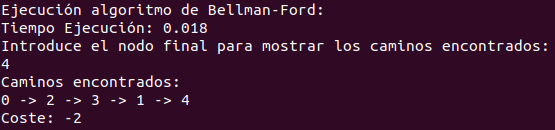
\includegraphics[width=12cm]{./Tiempos_Ejecucion/Ejecucion_BF}
	\end{subfigure}
	
	\caption{Resultado de ejecución del algoritmo BF con el grafo de la \autoref{fig:bell-ford}.}
	\label{fig:resultado_BF}
\end{figure}

\subsection{Resultado algoritmos de multiplicación de matrices}

\begin{figure}[!htb]
	\centering
	\begin{subfigure}{\linewidth}
		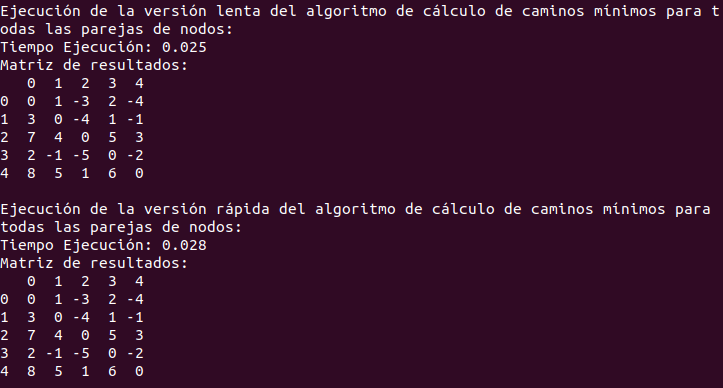
\includegraphics[width=12cm]{./Tiempos_Ejecucion/Ejecucion_Matrices}
	\end{subfigure}
	
	\caption{Resultado de ejecución de los algoritmos de multiplicación de matrices con el grafo de la \autoref{fig:3.4.1}.}
	\label{fig:resultado_Matrices}
\end{figure}

\newpage

\subsection{Resultado Floyd-Warshall}

En este caso se muestra además el camino encontrado entre el nodo $0$ y $1$, construido a partir de la matriz de predecesores.

\begin{figure}[!htb]
	\centering
	\begin{subfigure}{\linewidth}
		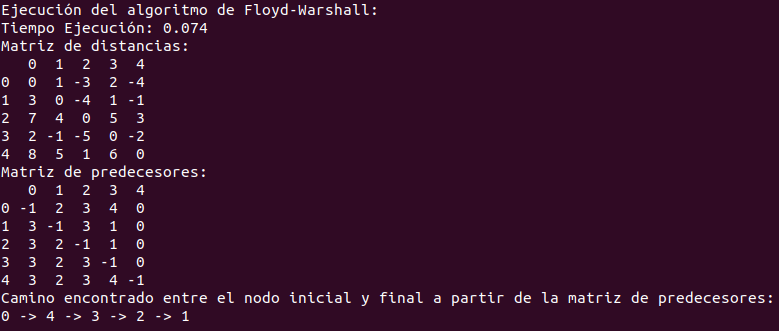
\includegraphics[width=12cm]{./Tiempos_Ejecucion/Ejecucion_FW}
	\end{subfigure}
	
	\caption{Resultado de ejecución del algoritmo de FW con el grafo de la \autoref{fig:3.4.1}.}
	\label{fig:resultado_FW}
\end{figure}

\subsection{Resultado clausura transitiva}

\begin{figure}[!htb]
	\centering
	\begin{subfigure}{\linewidth}
		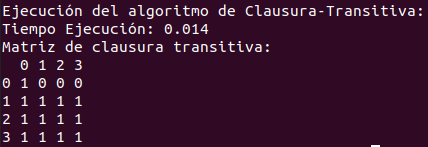
\includegraphics[width=12cm]{./Tiempos_Ejecucion/Ejecucion_CT}
	\end{subfigure}
	
	\caption{Resultado de ejecución del algoritmo de la clausura transitiva con el grafo de la \autoref{fig:claus-trans}.}
	\label{fig:resultado_CT}
\end{figure}

\section{Medición de tiempos y comparación con la complejidad teórica}

Para calcular el tiempo de ejecución de los algoritmos, utilizamos la función \textit{clock()} de C++, que devuelve el número de \textit{ticks} transcurridos desde una época relativa a la ejecución del programa. Ejecutando dicha función antes y después de llamar a la función que implementa el algoritmo y calculando la diferencia conseguimos el tiempo de ejecución. En este caso se ha medido en milisegundos. \\

Ya hemos comentado cómo se extraen los tiempos de un algoritmo concreto a partir del programa principal \textit{Tiempos.cpp}. Para extraer los tiempos de todos los algoritmos, se ha programado un script de bash, llamado \textit{calculo\_tiempos.sh}, situado en la carpeta \textit{bin}. Dicho script ejecuta y guarda en un archivo los tiempos de ejecución de cada algoritmo para $10$ números de nodos distintos, incrementándolos en cada ejecución. \\

Otro detalle importante es cómo medir el tamaño, pues tenemos dos cantidades, $|V|$ y $|E|$, y para ajustar la complejidad, necesitamos que la función dependa de una única variable. Para ello, utilizamos la densidad para escribir el número de aristas en función del número de vértices, y escogemos una densidad fija para calcular todos los tiempos. En este caso se ha escogido una desidad de $0.1$, aunque no tiene mucha importancia el número en concreto. \\

Una vez obtenidos los tiempos, que se guardan en la carpeta \textit{Resultados}, podemos mostrarlos utilizando la función \textit{plot} de Gnuplot. Las figuras \autoref{fig:tiempos_BFS} - \autoref{fig:tiempos_Todos} muestran las gráficas obtenidas mediante esta función, que representan los tiempos de ejecución de cada algoritmo en milisegundos en función del número de vértices. \\

\begin{figure}[!htb]
	\centering
	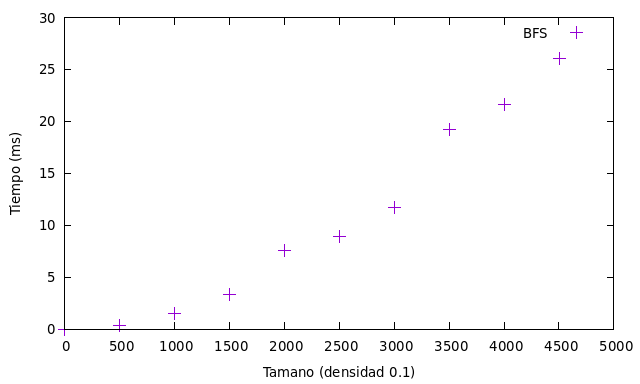
\includegraphics[width=9cm]{./Tiempos_Ejecucion/Tiempos_BFS_0.1}
	
	\caption{Tiempos de ejecución BFS.}
	\label{fig:tiempos_BFS}
\end{figure}

\begin{figure}[!htb]
	\centering
	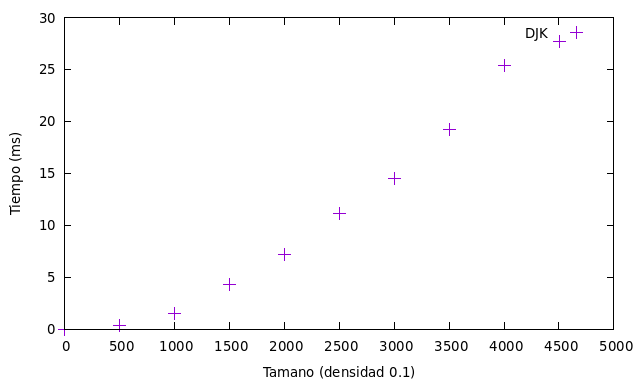
\includegraphics[width=9cm]{./Tiempos_Ejecucion/Tiempos_DJK_0.1}
	
	\caption{Tiempos de ejecución Dijkstra.}
	\label{fig:tiempos_DJK}
\end{figure}

\begin{figure}[!htb]
	\centering
	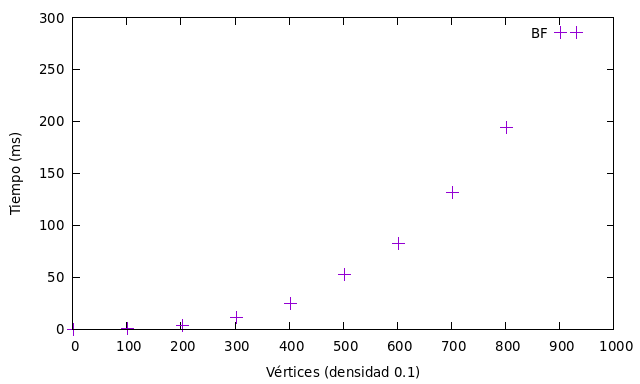
\includegraphics[width=9cm]{./Tiempos_Ejecucion/Tiempos_BF}
	
	\caption{Tiempos de ejecución Bellman-Ford.}
	\label{fig:tiempos_BF}
\end{figure}

\begin{figure}[!htb]
	\centering
	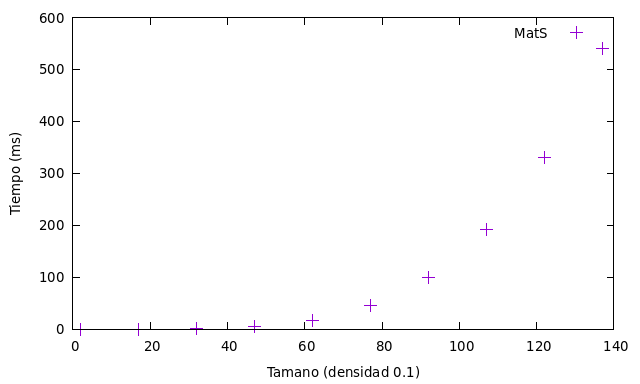
\includegraphics[width=9cm]{./Tiempos_Ejecucion/Tiempos_MatS}
	
	\caption{Tiempos de ejecución algoritmo de matrices lento.}
	\label{fig:tiempos_MatS}
\end{figure}

\begin{figure}[!htb]
	\centering
	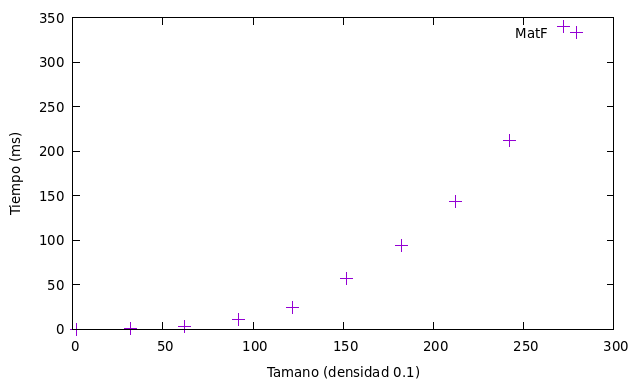
\includegraphics[width=9cm]{./Tiempos_Ejecucion/Tiempos_MatF}
	
	\caption{Tiempos de ejecución algoritmo de matrices rápido.}
	\label{fig:tiempos_MatF}
\end{figure}

\begin{figure}[!htb]
	\centering
	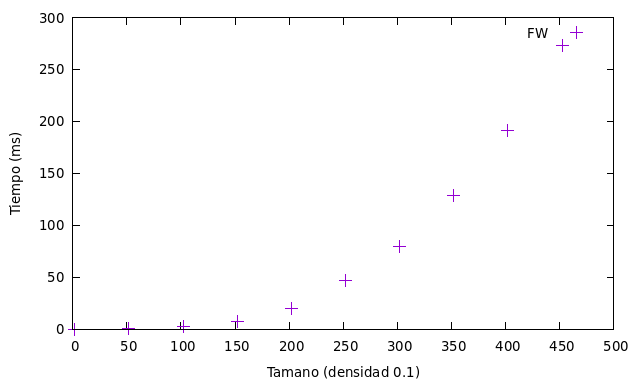
\includegraphics[width=9cm]{./Tiempos_Ejecucion/Tiempos_FW}
	
	\caption{Tiempos de ejecución Floyd-Warshall.}
	\label{fig:tiempos_FW}
\end{figure}

\begin{figure}[!htb]
	\centering
	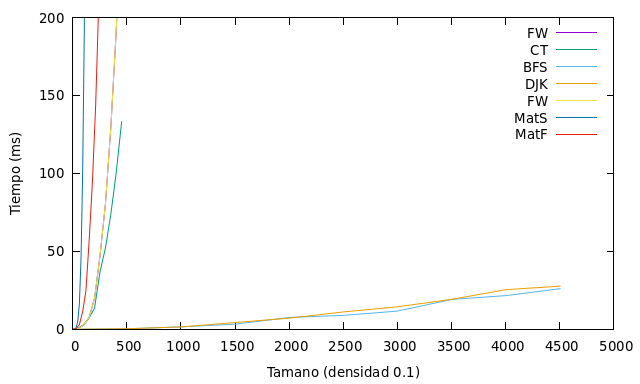
\includegraphics[width=9cm]{./Tiempos_Ejecucion/Tiempos_Todos}
	
	\caption{Tiempos de ejecución de todos los algoritmos.}
	\label{fig:tiempos_Todos}
\end{figure}

\subsection{Tiempo de ejecución de los algoritmos BFS y Dijkstra}

\begin{figure}[htb]
	\centering
	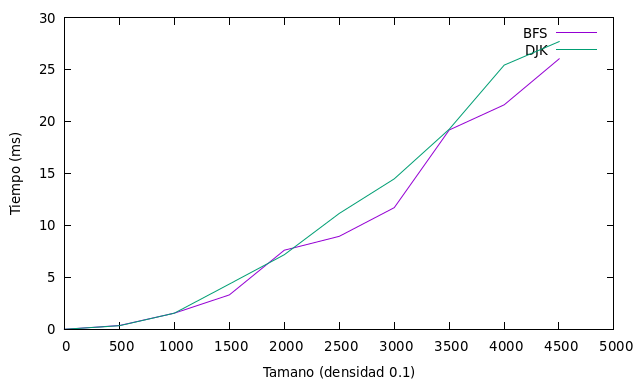
\includegraphics[width=7cm]{./Tiempos_Ejecucion/Tiempos_BFS_DJK_0.1}
	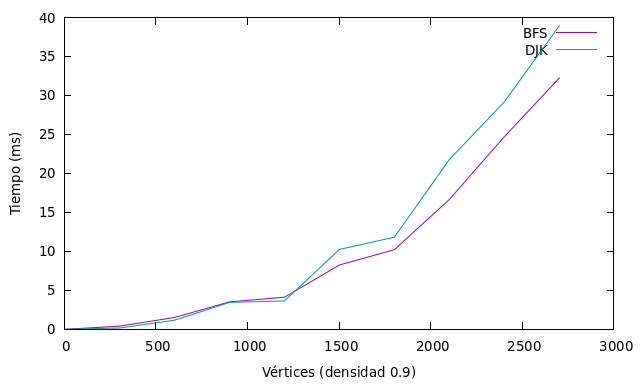
\includegraphics[width=7cm]{./Tiempos_Ejecucion/Tiempos_BFS_DJK_0.9}
	
	\caption{Comparación entre los tiempos de ejecución del algoritmo BFS y Dijkstra para distintas densidades de grafos.}
	\label{fig:BFS_DJK}
\end{figure}

En este apartado vamos a comentar un curioso resultado obtenido tras probar con diferentes densidades de grafos. Si observamos la implementación del algoritmo de Dijkstra, la única diferencia con BFS es el uso de la cola con prioridad, cuya operación de inserción tiene complejidad igual al logaritmo del tamaño de la cola. Esto hace que, sobre grafos dispersos, como la cola no suele estar muy llena, esta operación sea relativamente rápida, consiguiendo por tanto tiempos muy similares a BFS, esta diferencia se puede apreciar en las gráficas de la \autoref{fig:BFS_DJK} , donde se han extraído tiempos para densidades de grafo de $0.1$ y $0.9$.

\subsection{Tiempo de ejecución de los algoritmos Floyd-Warshal y de clausura transitiva}

Mostramos aquí la comparación entre los tiempos de ejecución del algoritmo de Floyd-Warshall y la clausura transitiva, para comprobar como, efectivamente, el uso de variables booleanas y funciones lógicas es menos costoso en tiempo, para ello en la \autoref{fig:FW_CT} mostramos un gráfico con los tiempos de ejecución de ambos algoritmos.

\begin{figure}[htb]
	\centering
	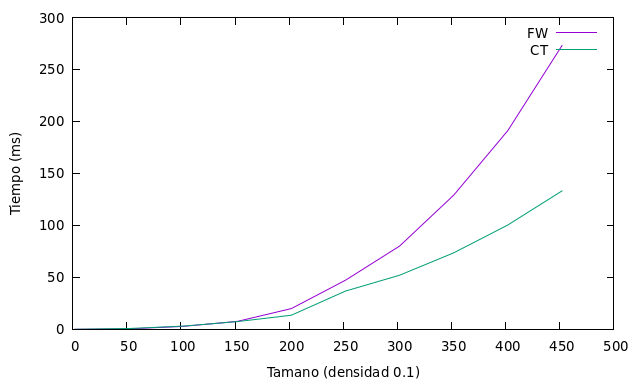
\includegraphics[width=7cm]{./Tiempos_Ejecucion/Tiempos_FW_CT}
	
	\caption{Comparación entre los tiempos de ejecución del algoritmo de Floyd-Warshall y la clausura transitiva.}
	\label{fig:FW_CT}
\end{figure}

\subsection{Contraste con la complejidad teórica}

Para llevar a cabo este contraste se ha utilizado la función \textit{fit} de Gnuplot, que ajusta una función creada a una serie de puntos. El proceso a seguir es simple, se crea una función que represente la complejidad teórica y se ajusta a los resultados obtenidos. Si la función ajusta bien los resultados obtenidos, entonces podemos concluir que la complejidad teórica es correcta. \\

La función a crear depende de la complejidad, por ejemplo, si la complejidad es $O(V^2)$, la función a ajustar sería $f(x) = a_0x^2 + a_1$. Ya hemos comentado que escribimos el número de aristas en función del número de vértices. Por ello, en el caso de ser complejidad $O(E)$, por ejemplo, la función sería $f(x) = a_0x(x-1)0.1 + a_1$, pues la densidad la hemos fijado a $0.1$. \\ 

En las figuras \autoref{fig:ajuste_BFS} - \autoref{fig:ajuste_FW} se pueden ver las gráficas de las funciones ajustadas superpuestas con los tiempos de ejecución junto a la función ajustada y la complejidad teórica. Se puede observar como todas las complejidades son correctas.\\

\newpage

Complejidad: $O(V+E)$, función: $f(x) = a_0x + a_1x(x-1)0.1 + a_2$

\begin{figure}[!htb]
	\centering
	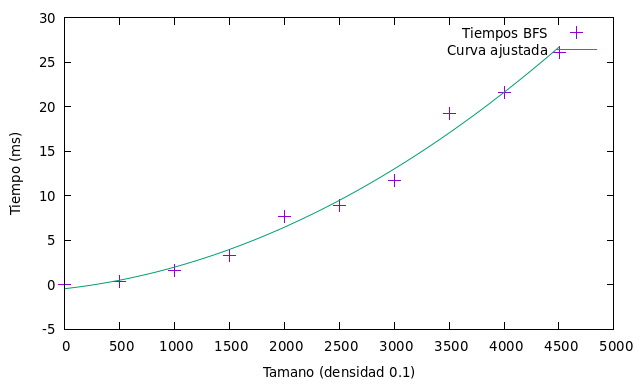
\includegraphics[width=8.5cm]{./Tiempos_Ejecucion/Ajuste_BFS}
	
	\caption{Ajuste de la complejidad del algoritmo BFS.}
	\label{fig:ajuste_BFS}
\end{figure}


Complejidad: $O((V+E)log(V))$, función: $f(x) = (a_0x + a_1x(x-1)0.1)a_2log(x) + a_3$

\begin{figure}[!htb]
	\centering
	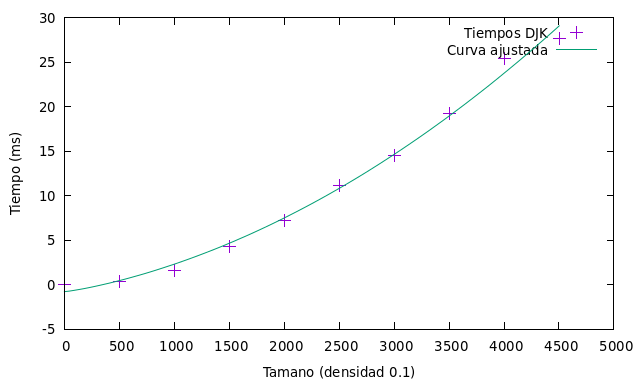
\includegraphics[width=8.5cm]{./Tiempos_Ejecucion/Ajuste_DJK}
	
	\caption{Ajuste de la complejidad del algoritmo de Dijkstra.}
	\label{fig:ajuste_DJK}
\end{figure}


Complejidad: $O(VE)$, función: $f(x) = a_0xa_1x(x-1)0.1 + a_2$

\begin{figure}[!htb]
	\centering
	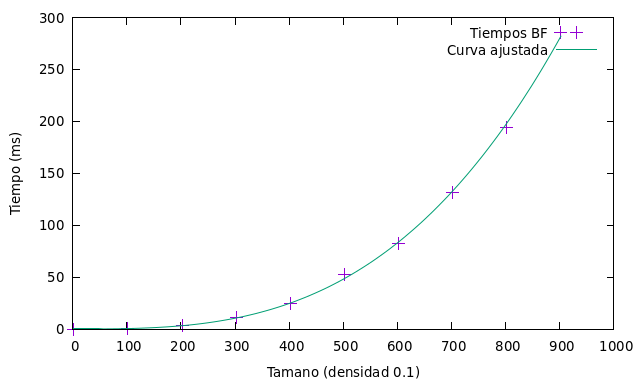
\includegraphics[width=8.5cm]{./Tiempos_Ejecucion/Ajuste_BF}
	
	\caption{Ajuste de la complejidad del algoritmo de Bellman-Ford.}
	\label{fig:ajuste_BF}
\end{figure}

\newpage

Complejidad: $O(V^4)$, función: $f(x) = a_0x^4 + a_1$

\begin{figure}[!htb]
	\centering
	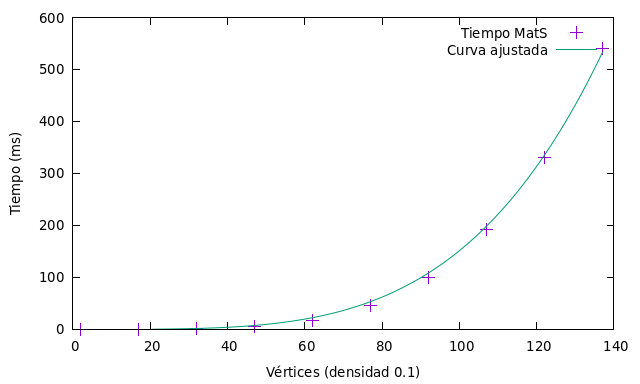
\includegraphics[width=8.5cm]{./Tiempos_Ejecucion/Ajuste_MatS}
	
	\caption{Ajuste de la complejidad del algoritmo de matrices lento.}
	\label{fig:ajuste_MatS}
\end{figure}

Complejidad: $O(V^3log(V))$, función: $f(x) = a_0x^3 + a_1log(x) + a_2$

\begin{figure}[!htb]
	\centering
	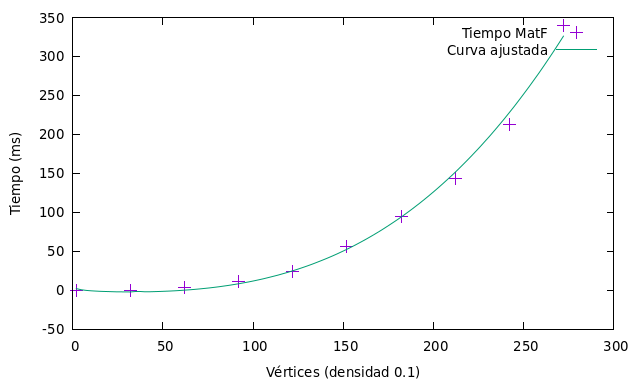
\includegraphics[width=8.5cm]{./Tiempos_Ejecucion/Ajuste_MatF}
	
	\caption{Ajuste de la complejidad del algoritmo de matrices rápido.}
	\label{fig:ajuste_MatF}
\end{figure}

Complejidad: $O(V^3)$, función: $f(x) = a_0x^3 + a_1$

\begin{figure}[!htb]
	\centering
	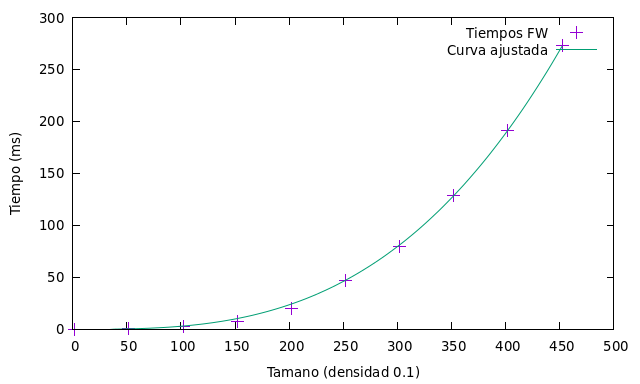
\includegraphics[width=8.5cm]{./Tiempos_Ejecucion/Ajuste_FW}
	
	\caption{Ajuste de la complejidad del algoritmo de Floyd-Warshall.}
	\label{fig:ajuste_FW}
\end{figure}

\endinput



